\documentclass[letterpaper,11pt]{article}
\usepackage{graphicx}
\usepackage{listings}
\usepackage[super]{nth}
\usepackage[hyphens]{url}
\usepackage{hyperref}
\usepackage{amsmath}
\usepackage[makeroom]{cancel}
\usepackage[table]{xcolor}
\usepackage{comment}
\usepackage[space]{grffile}
\usepackage{csvsimple}
\usepackage{longtable}


\newcommand*{\srcPath}{../src}%

\lstset{
	basicstyle=\footnotesize,
	breaklines=true,
}

\begin{document}

\begin{titlepage}

\begin{center}

\Huge{Assignment 8}

\Large{CS 532:  Introduction to Web Science}

\Large{Spring 2017}

\Large{Grant Atkins}

\Large Finished on \today

\end{center}

\end{titlepage}

\newpage


% =================================
% First question
% =================================
\section*{1}

\subsection*{Question}

\begin{verbatim}
1.  Create a blog-term matrix.  Start by grabbing 100 blogs; include:

http://f-measure.blogspot.com/
http://ws-dl.blogspot.com/

and grab 98 more as per the method shown in class.  Note that this
method randomly chooses blogs and each student will separately do
this process, so it is unlikely that these 98 blogs will be shared
among students.  In other words, no sharing of blog data.  Upload
to github your code for grabbing the blogs and provide a list of
blog URIs, both in the report and in github.

Use the blog title as the identifier for each blog (and row of the
matrix).  Use the terms from every item/title (RSS) or entry/title
(Atom) for the columns of the matrix.  The values are the frequency
of occurrence.  Essentially you are replicating the format of the
"blogdata.txt" file included with the PCI book code.  Limit the
number of terms to the most "popular" (i.e., frequent) 1000 terms,
this is *after* the criteria on p. 32 (slide 7) has been satisfied.
Remember that blogs are paginated. 
\end{verbatim}

\clearpage
\subsection*{Answer}

First approaching this problem I decided to use the tweepy library for python 3.6 to retrieve a json formatted list of Dr. Nelson's followers, which for me at the time was 634 followers, which was then saved to a file named \textbf{phonedudeFollowers.json} using the python script \textbf{getFollowers.py} shown in Listing \ref{lst:getFollowers.py}. Then I decided to reduce the number of friendships to check since checking friendships between all 634 followers would have been fairly time consuming. Therefore I created another script called \textbf{chooseUsers.py} which would pick 100 random integers for numbers between 1 and 634, which would act as which line numbers I would choose to sample from the json followers I retrieved earlier. This method actually worked out very well because I ended up getting quite a few members that were actually at Old Dominion University, as shown in Table \ref{table:q1userschosen}, without me tampering with it at all - however I may have run it a few times to test it.

I then took the 100 followers I had just chosen, added Dr. Nelson's user name $phonedude\_mln$, and continued to use tweepy again to check friendships between this list of users using the python script \textbf{findFriendships.py} shown in Listing \ref{lst:friendships.py}. It should be noted that I first decided to minimize the number of api calls by reducing the pairs I had to check. This was done by the \textit{minimizeConnections} function, which mapped all users as keys with values of every other user that was not already a key. This reduced the number of api calls from 10100 to 5150, with more logic explained in that function starting on line 14. This script took a several hours due to Twitter's rate limits. When it was completed all the friendships to each other user was saved to \textbf{friendships.csv} in the format of:

\begin{table}[htb]
\centering
\begin{tabular}{ | l | l | l | l |}
\hline
\textbf{Source User} & \textbf{Target User} & \textbf{Following Target} & \textbf{Followed By Target} \\
\hline
\end{tabular}
\caption{Format of friendships.csv, where Following fields are booleans}
\label{table:q1csvtable}
\end{table}

Finally to utilize D3.js to its utmost, I decided to convert the csv data and json data saved earlier, to create a new formatted json data with two main keys: nodes and links. To accomplish this I created a script named \textbf{createGraphJson.py}, so the data could properly represent a force directed graph. The all followers graph shown in Figure \ref{fig:q1allfollwersgraph} and the friendship graph of the 100 users generated shown in Figure \ref{fig:q1friendshipgraph} were generated using D3 using the \textit{drawGraph} function defined in \textbf{twitterFriendship.js} shown in Listing \ref{lst:q1javascript}. On hover a side bar should appear showing the user's name, user id, and profile image which links to the associated account. It should be noted that 1 user on the friendship graph is disconnected because when tweepy checked the account it was actually suspended by the time it got to it, making friendships impossible to establish. These two visualizations can be found here:

\url{https://cdn.rawgit.com/grantat/cs532-s17/b410d0d7/assignments/A6/src/index.html}


\clearpage
 \begin{figure}[h]
 \centering
 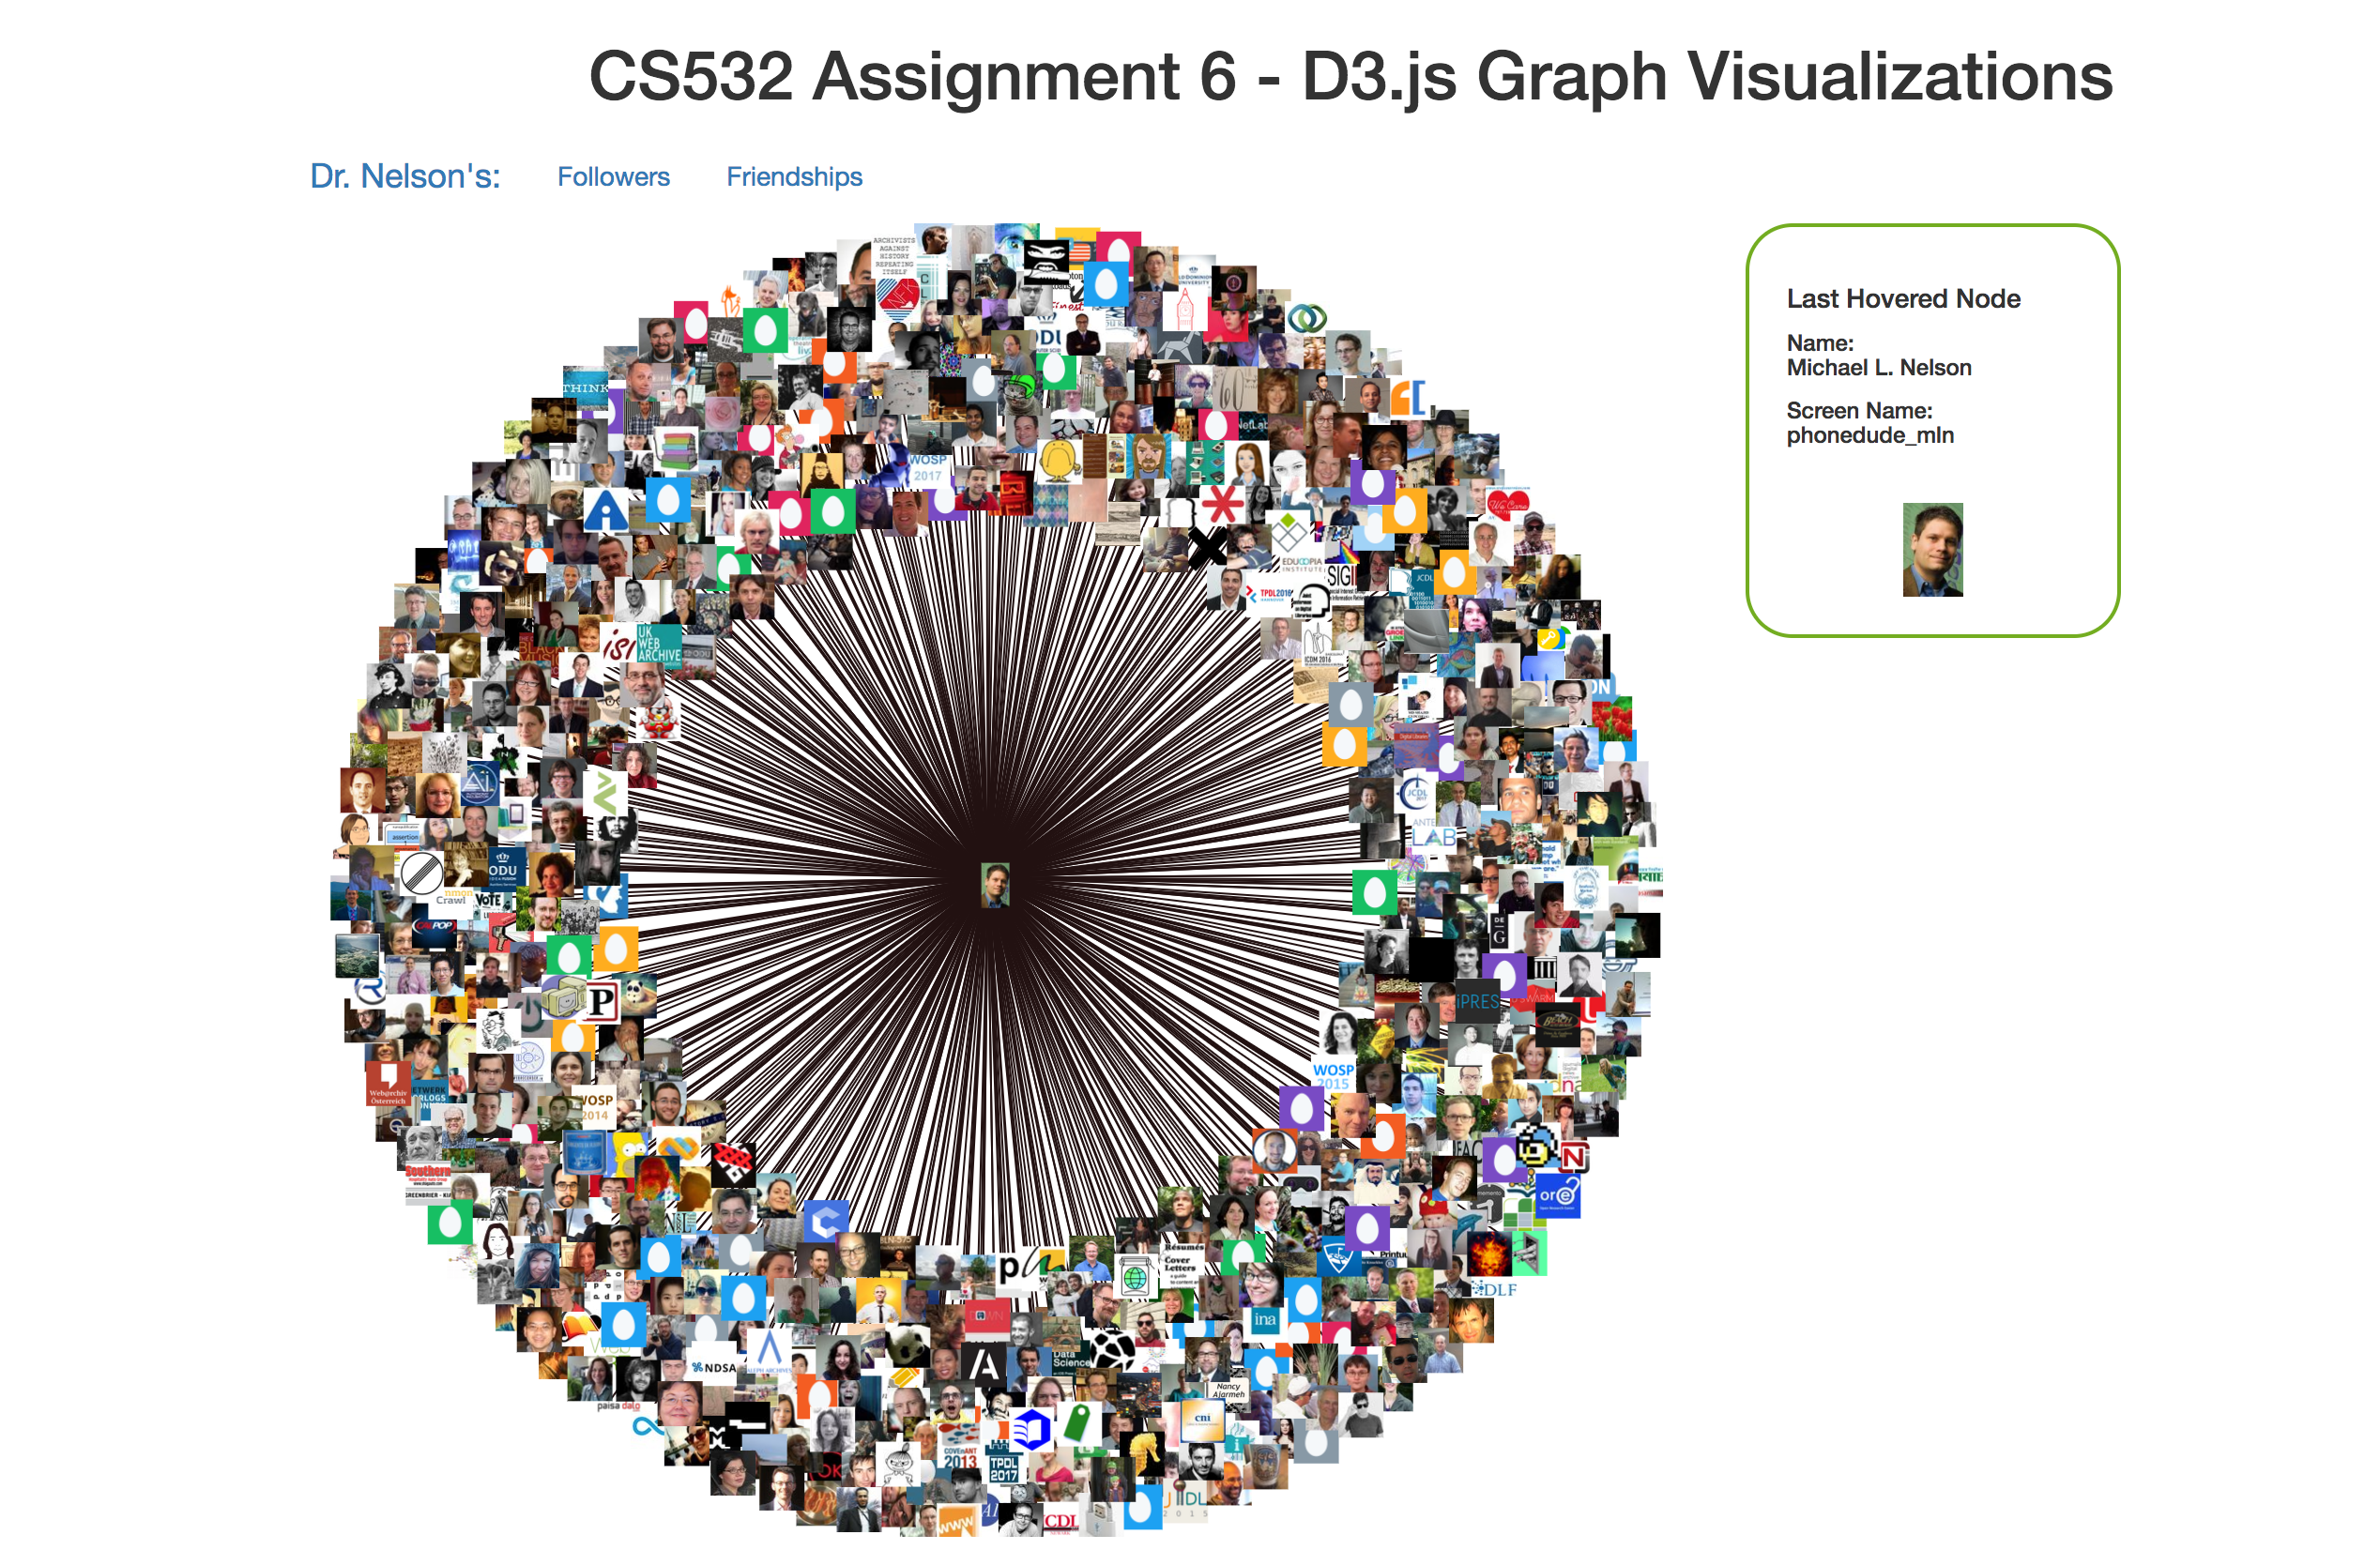
\includegraphics[scale=0.4]{d3followerGraph.png}
 \caption{All of Dr. Nelson's followers in D3 force directed graph}
 \label{fig:q1friendshipgraph}
 \end{figure}

\clearpage
 \begin{figure}[h]
 \centering
 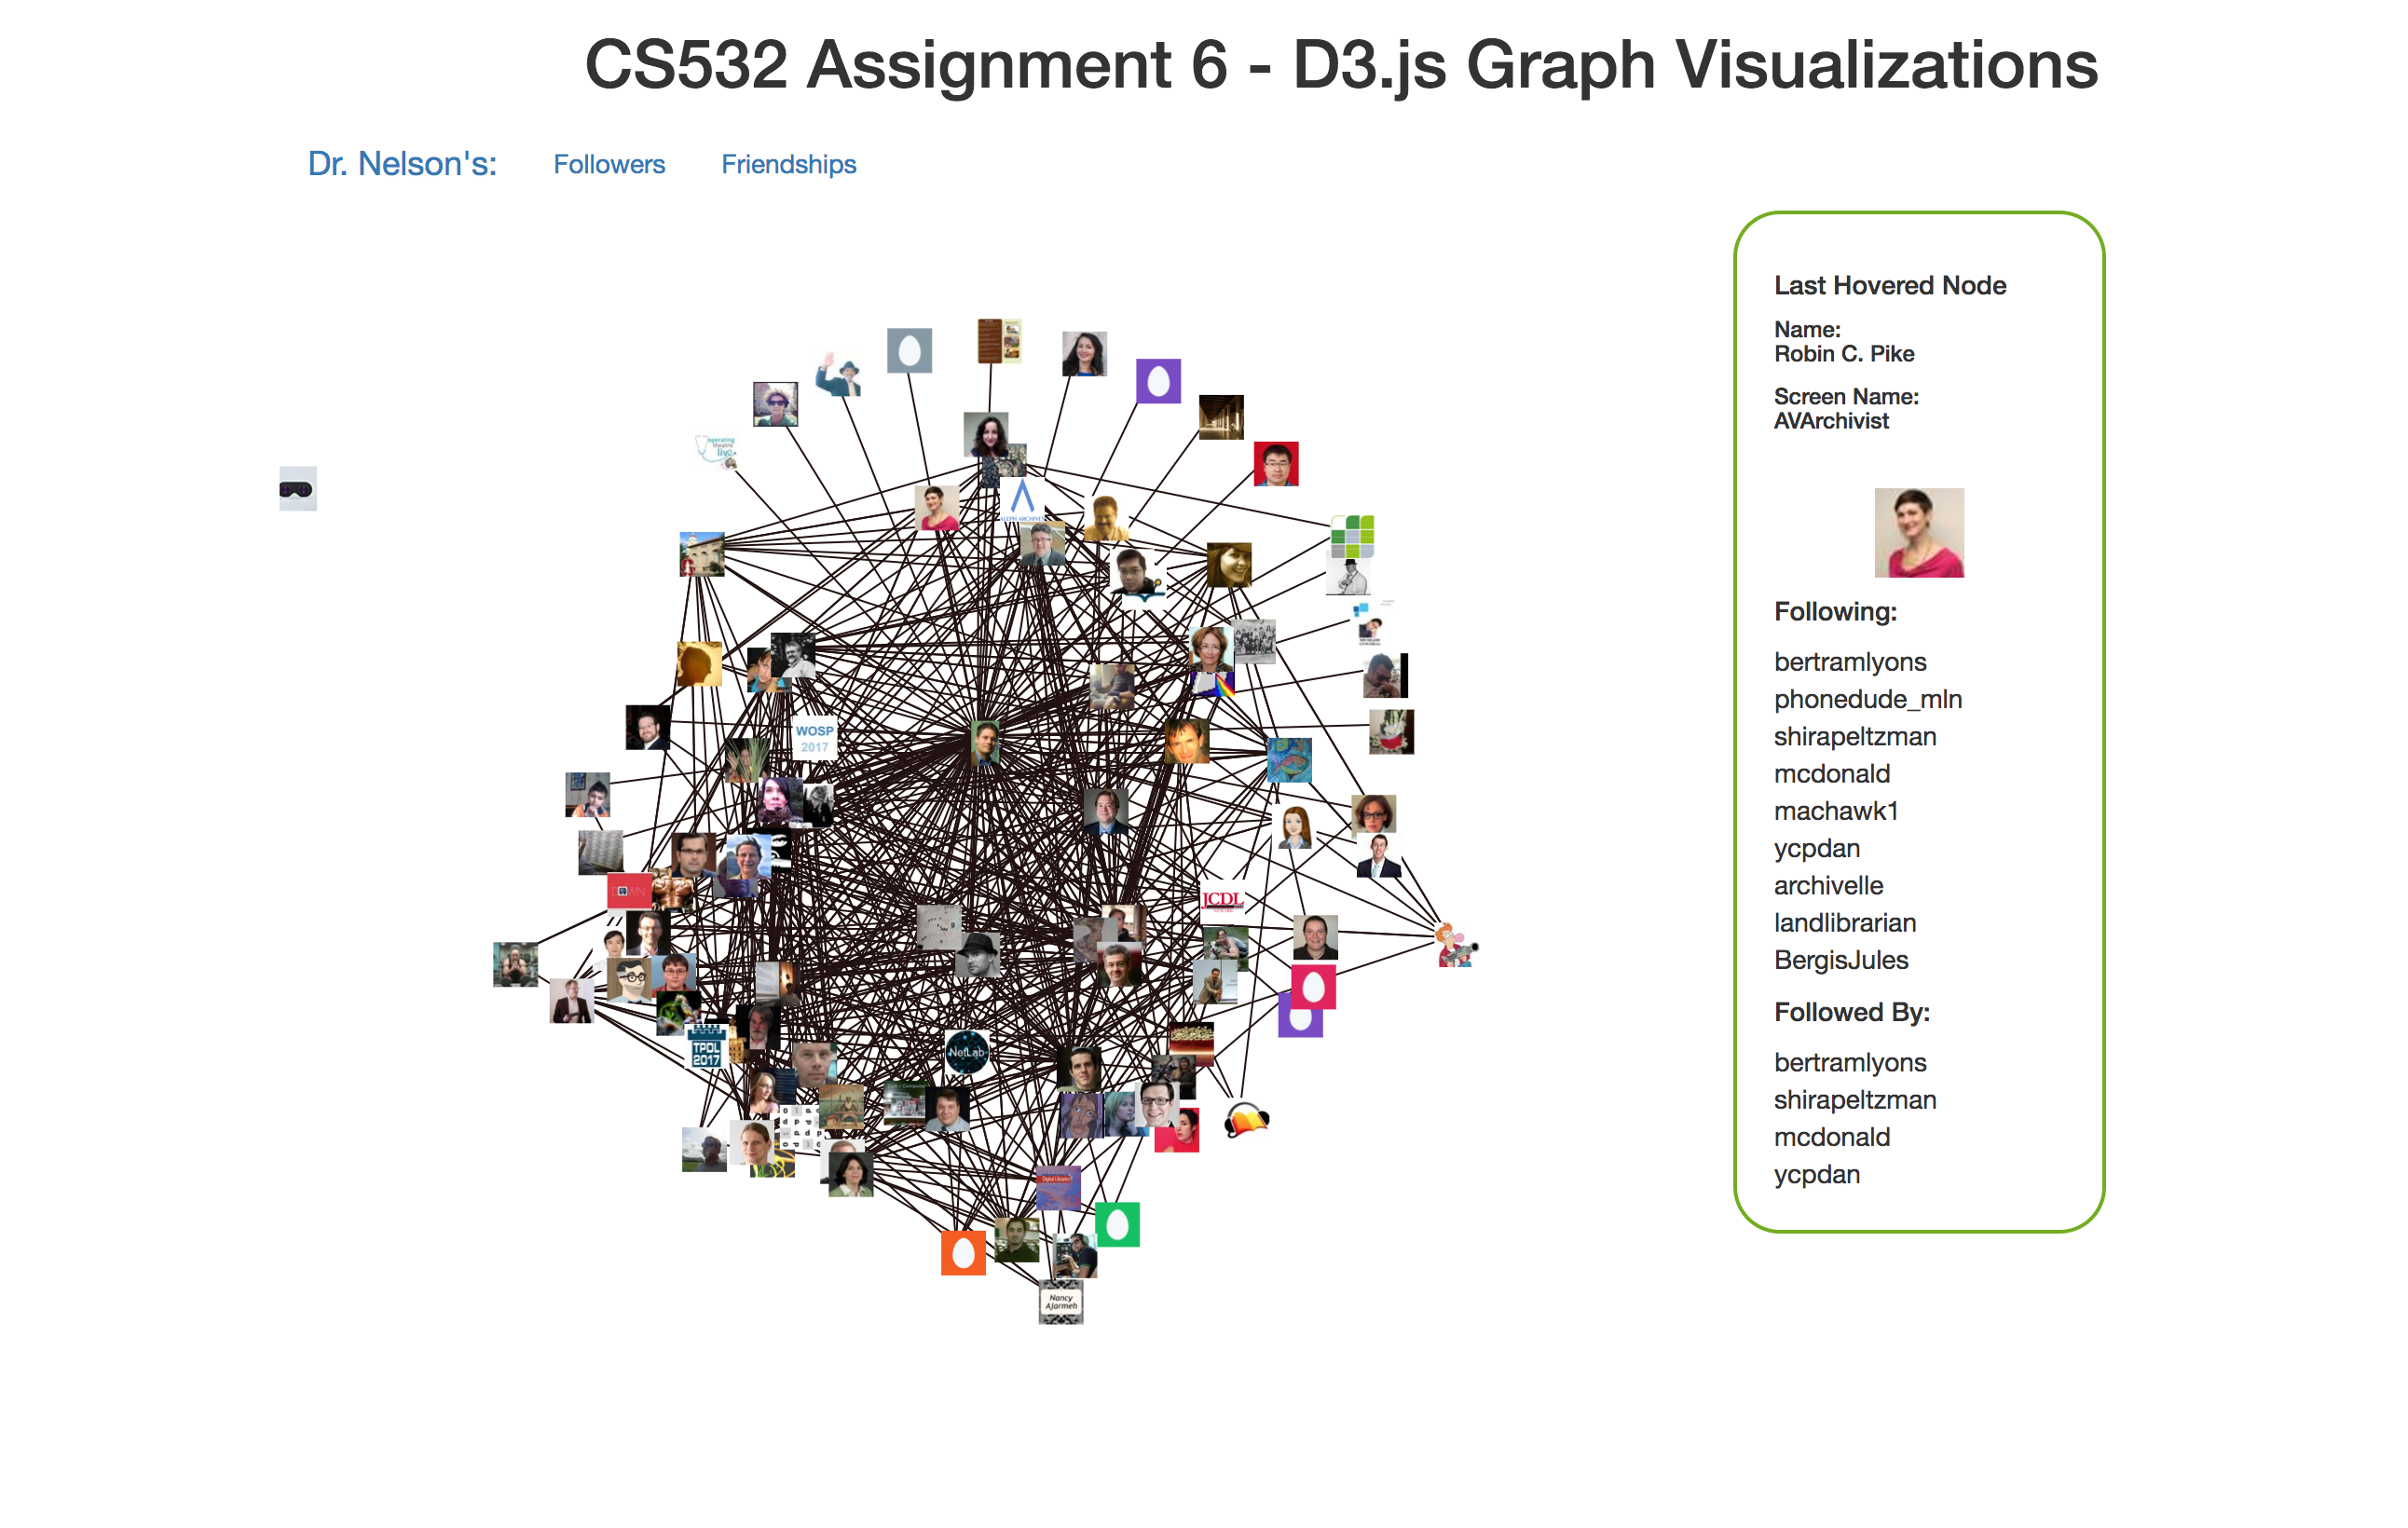
\includegraphics[scale=0.4]{d3friendshipGraph.png}
 \caption{Friendships graph of 100 selected users}
 \label{fig:q1allfollwersgraph}
 \end{figure}

 \lstinputlisting[frame=single,caption={Python script to retrieve Dr. Nelson's followers},label=lst:getFollowers.py,captionpos=b,numbers=left,showspaces=false,showstringspaces=false,basicstyle=\footnotesize]{\srcPath/getFollowers.py}

 \lstinputlisting[frame=single,caption={Python script to check twitter friendships},label=lst:friendships.py,captionpos=b,numbers=left,showspaces=false,showstringspaces=false,basicstyle=\footnotesize]{\srcPath/findFriendships.py}

 \lstinputlisting[frame=single,caption={Javascript to create force directed graphs},label=lst:q1javascript,captionpos=b,numbers=left,showspaces=false,showstringspaces=false,basicstyle=\footnotesize]{\srcPath/js/twitterFriendships.js}

\clearpage

% =================================
% Second question
% =================================

\section*{2}

\subsection*{Question}

\begin{verbatim}
2.  Create an ASCII and JPEG dendrogram that clusters (i.e., HAC)
the most similar blogs (see slides 12 & 13).  Include the JPEG in
your report and upload the ascii file to github (it will be too
unwieldy for inclusion in the report).
\end{verbatim}

\subsection*{Answer}




% \begin{figure}[h]
% \centering
% 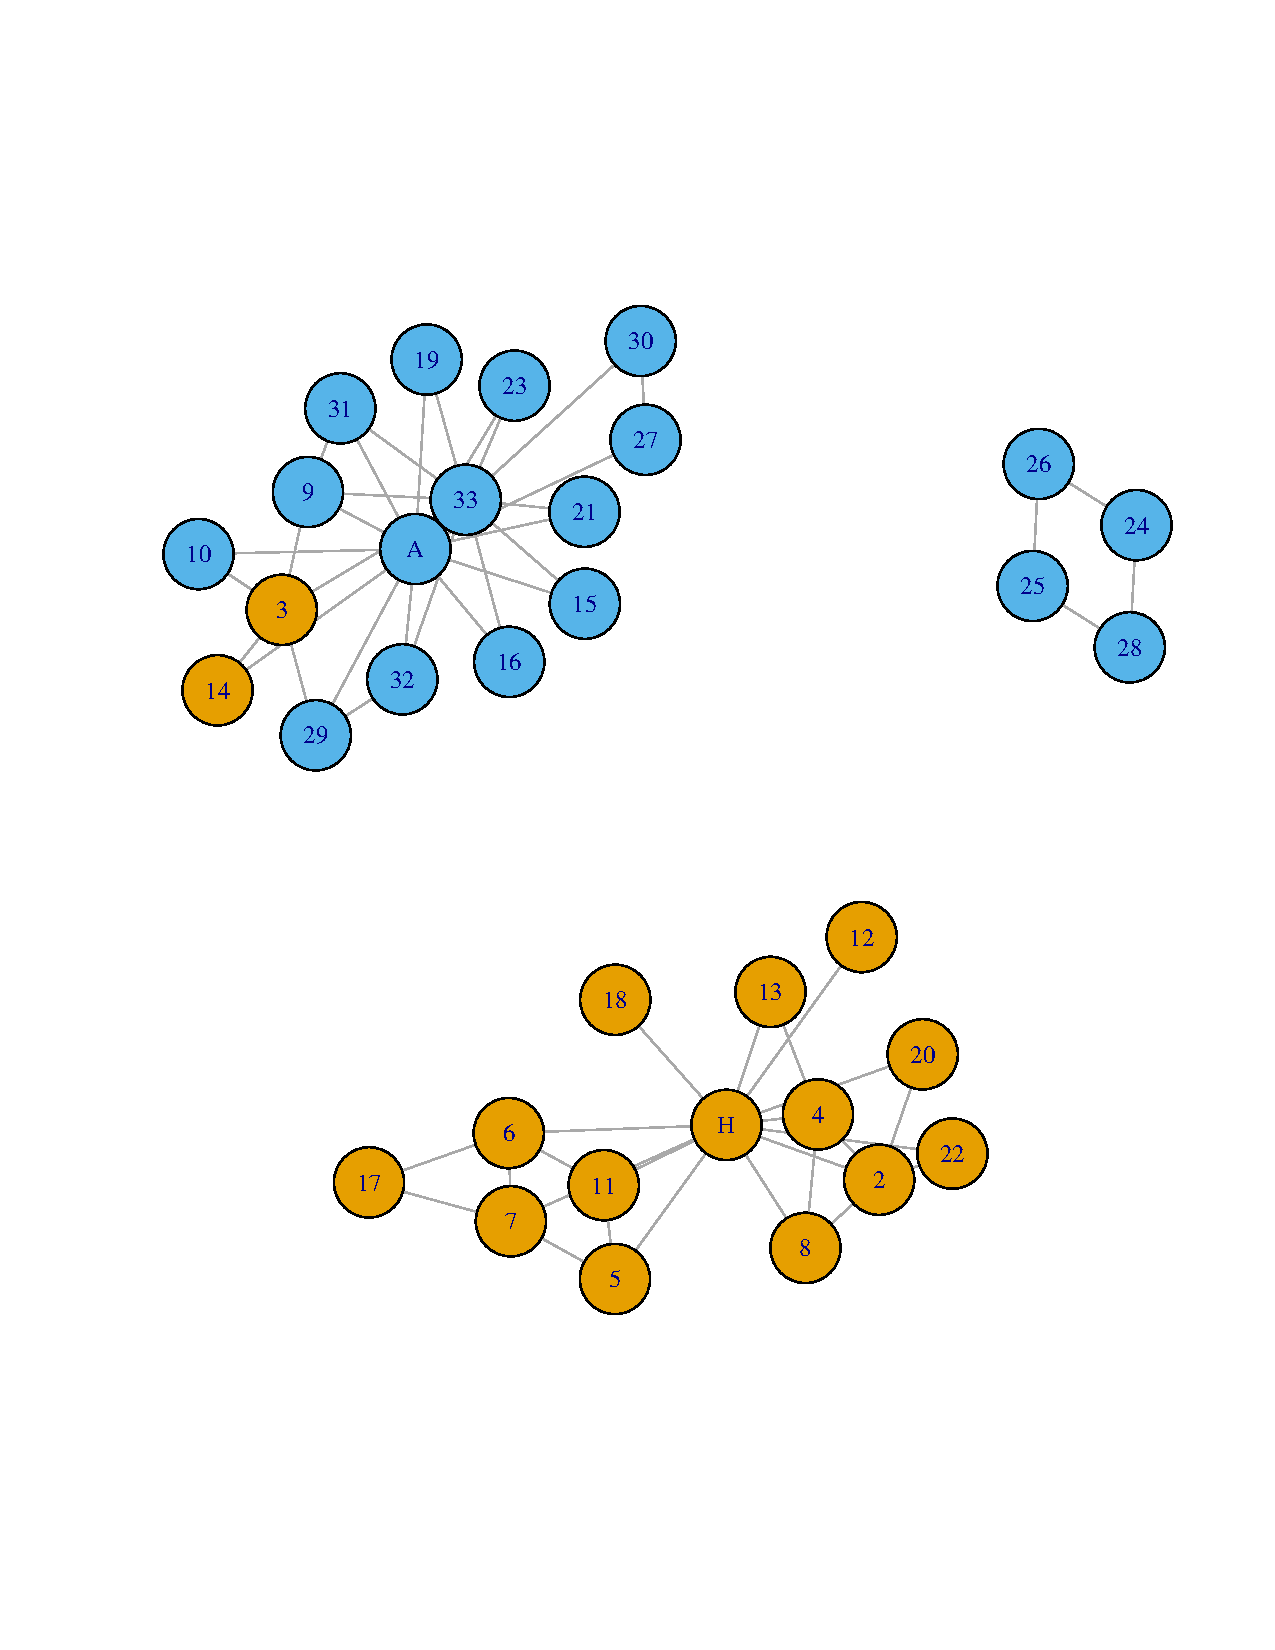
\includegraphics[scale=0.6]{predictedSplit3.pdf}
% \caption{Group split of 3 with Girvan-Newman algorithm from karateClub.R}
% \label{fig:split3}
% \end{figure}

\clearpage

% =================================
% 3rd question
% =================================

\section*{3}

\subsection*{Question}

\begin{verbatim}
3.  Cluster the blogs using K-Means, using k=5,10,20. (see slide
18).  Print the values in each centroid, for each value of k.  How
many interations were required for each value of k?
\end{verbatim}

\subsection*{Answer}

\begin{center}
\Huge{NOT ATTEMPTED}
\end{center}

% \begin{figure}[h]
% \centering
% 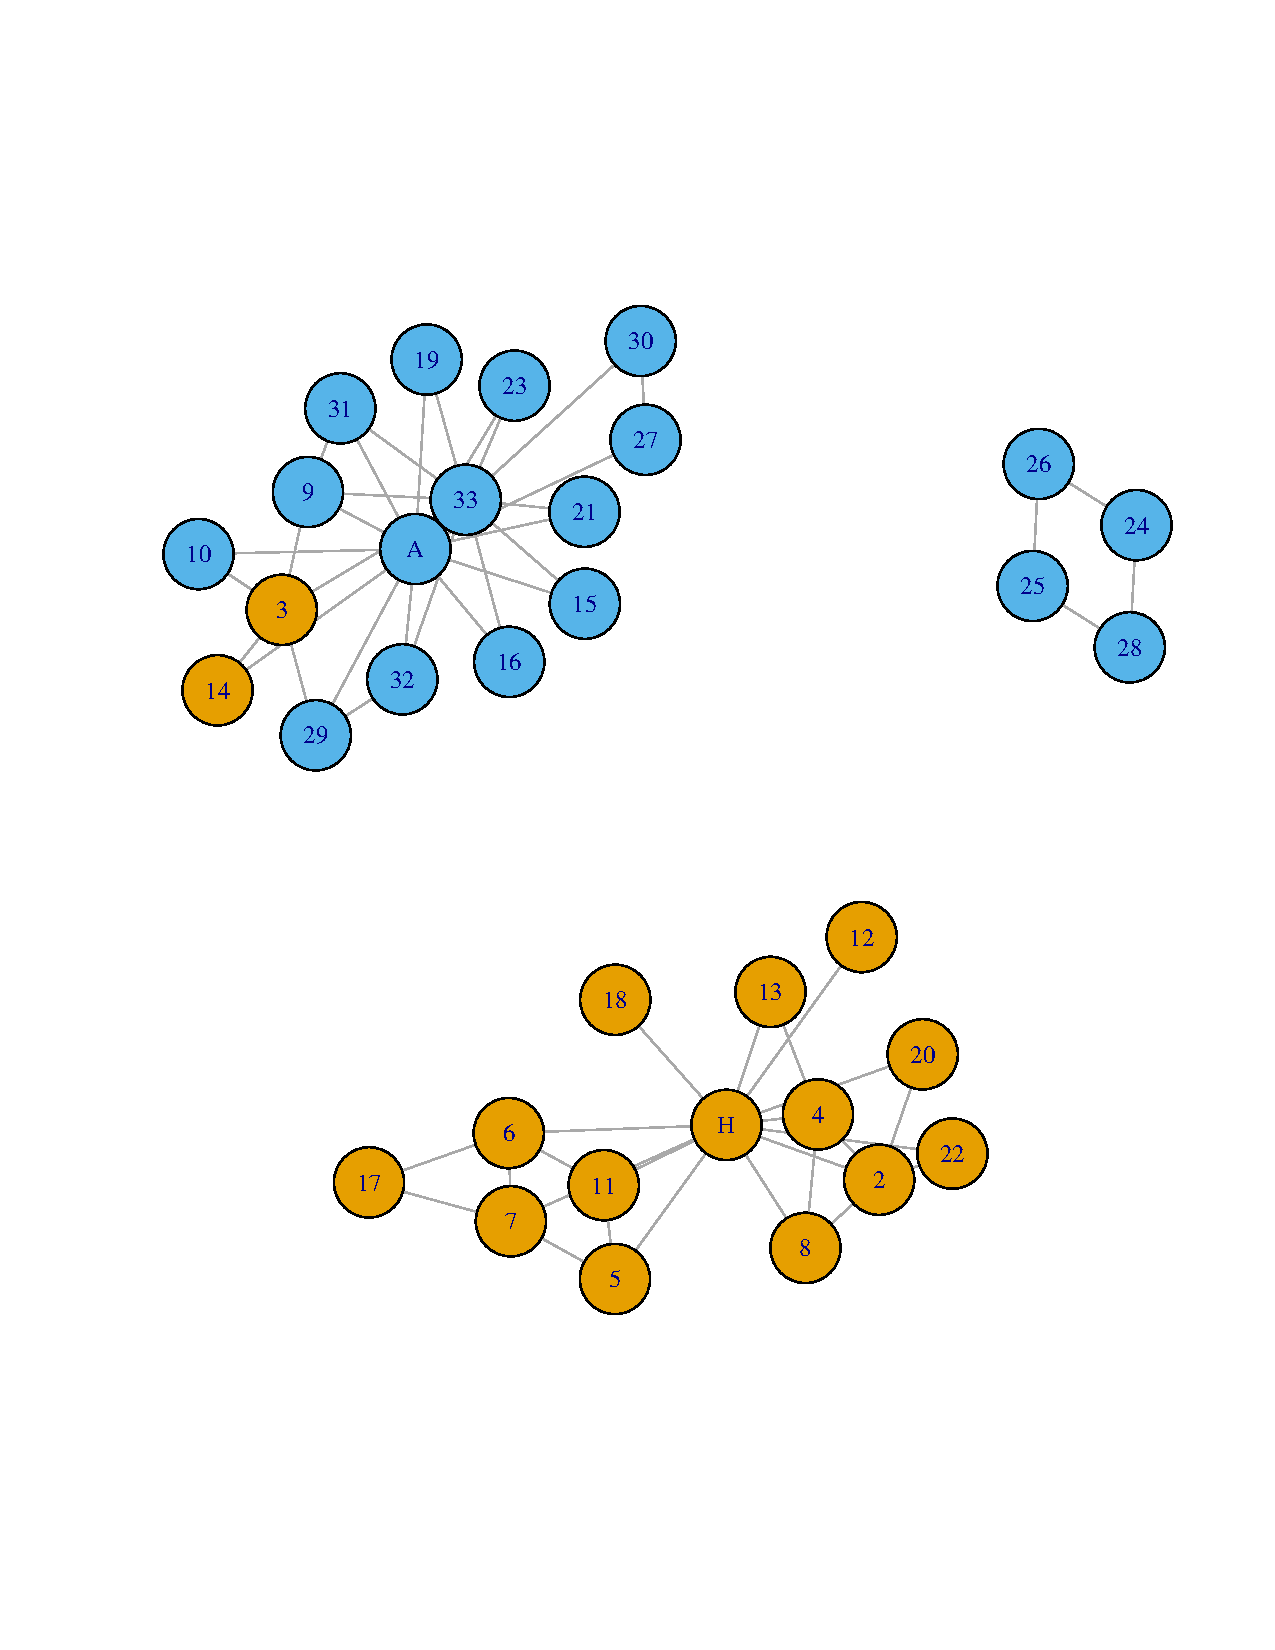
\includegraphics[scale=0.6]{predictedSplit3.pdf}
% \caption{Group split of 3 with Girvan-Newman algorithm from karateClub.R}
% \label{fig:split3}
% \end{figure}


% =================================
% 4th question
% =================================

\section*{4}

\subsection*{Question}

\begin{verbatim}
4.  Use MDS to create a JPEG of the blogs similar to slide 29 of the 
week 12 lecture.  How many iterations were required?
\end{verbatim}

\subsection*{Answer}

\begin{center}
\Huge{NOT ATTEMPTED}
\end{center}

% \begin{figure}[h]
% \centering
% 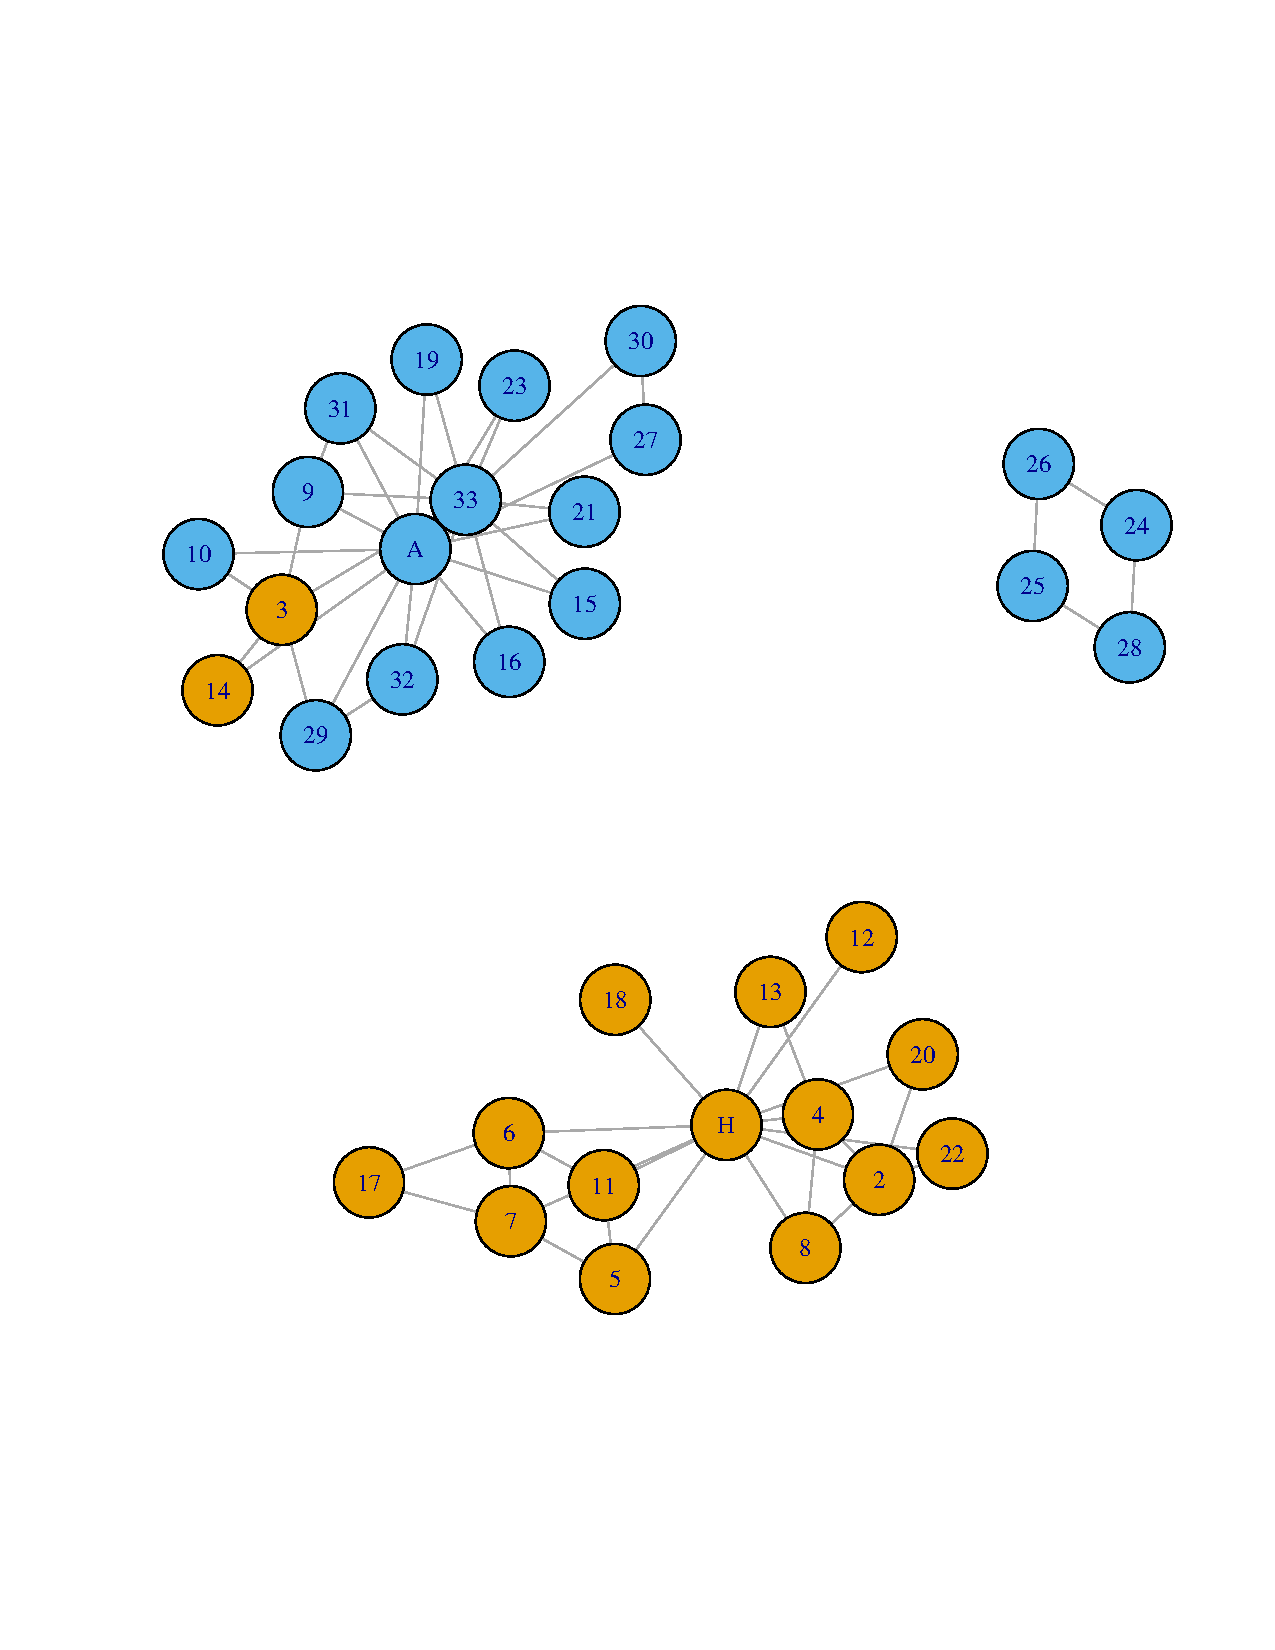
\includegraphics[scale=0.6]{predictedSplit3.pdf}
% \caption{Group split of 3 with Girvan-Newman algorithm from karateClub.R}
% \label{fig:split3}
% \end{figure}

\clearpage

% =================================
% Extra credit
% 5th question
% =================================

\section*{5}

\subsection*{Question}

\begin{verbatim}
5.  Re-run question 2, but this time with proper TFIDF calculations
instead of the hack discussed on slide 7 (p. 32).  Use the same 1000
words, but this time replace their frequency count with TFIDF scores
as computed in assignment #3.  Document the code, techniques,
methods, etc. used to generate these TFIDF values.  Upload the new
data file to github.

Compare and contrast the resulting dendrogram with the dendrogram
from question #2.

Note: ideally you would not reuse the same 1000 terms and instead
come up with TFIDF scores for all the terms and then choose the top
1000 from that list, but I'm trying to limit the amount of work
necessary.
\end{verbatim}

\subsection*{Answer}

\begin{center}
\Huge{NOT ATTEMPTED}
\end{center}

% \begin{figure}[h]
% \centering
% 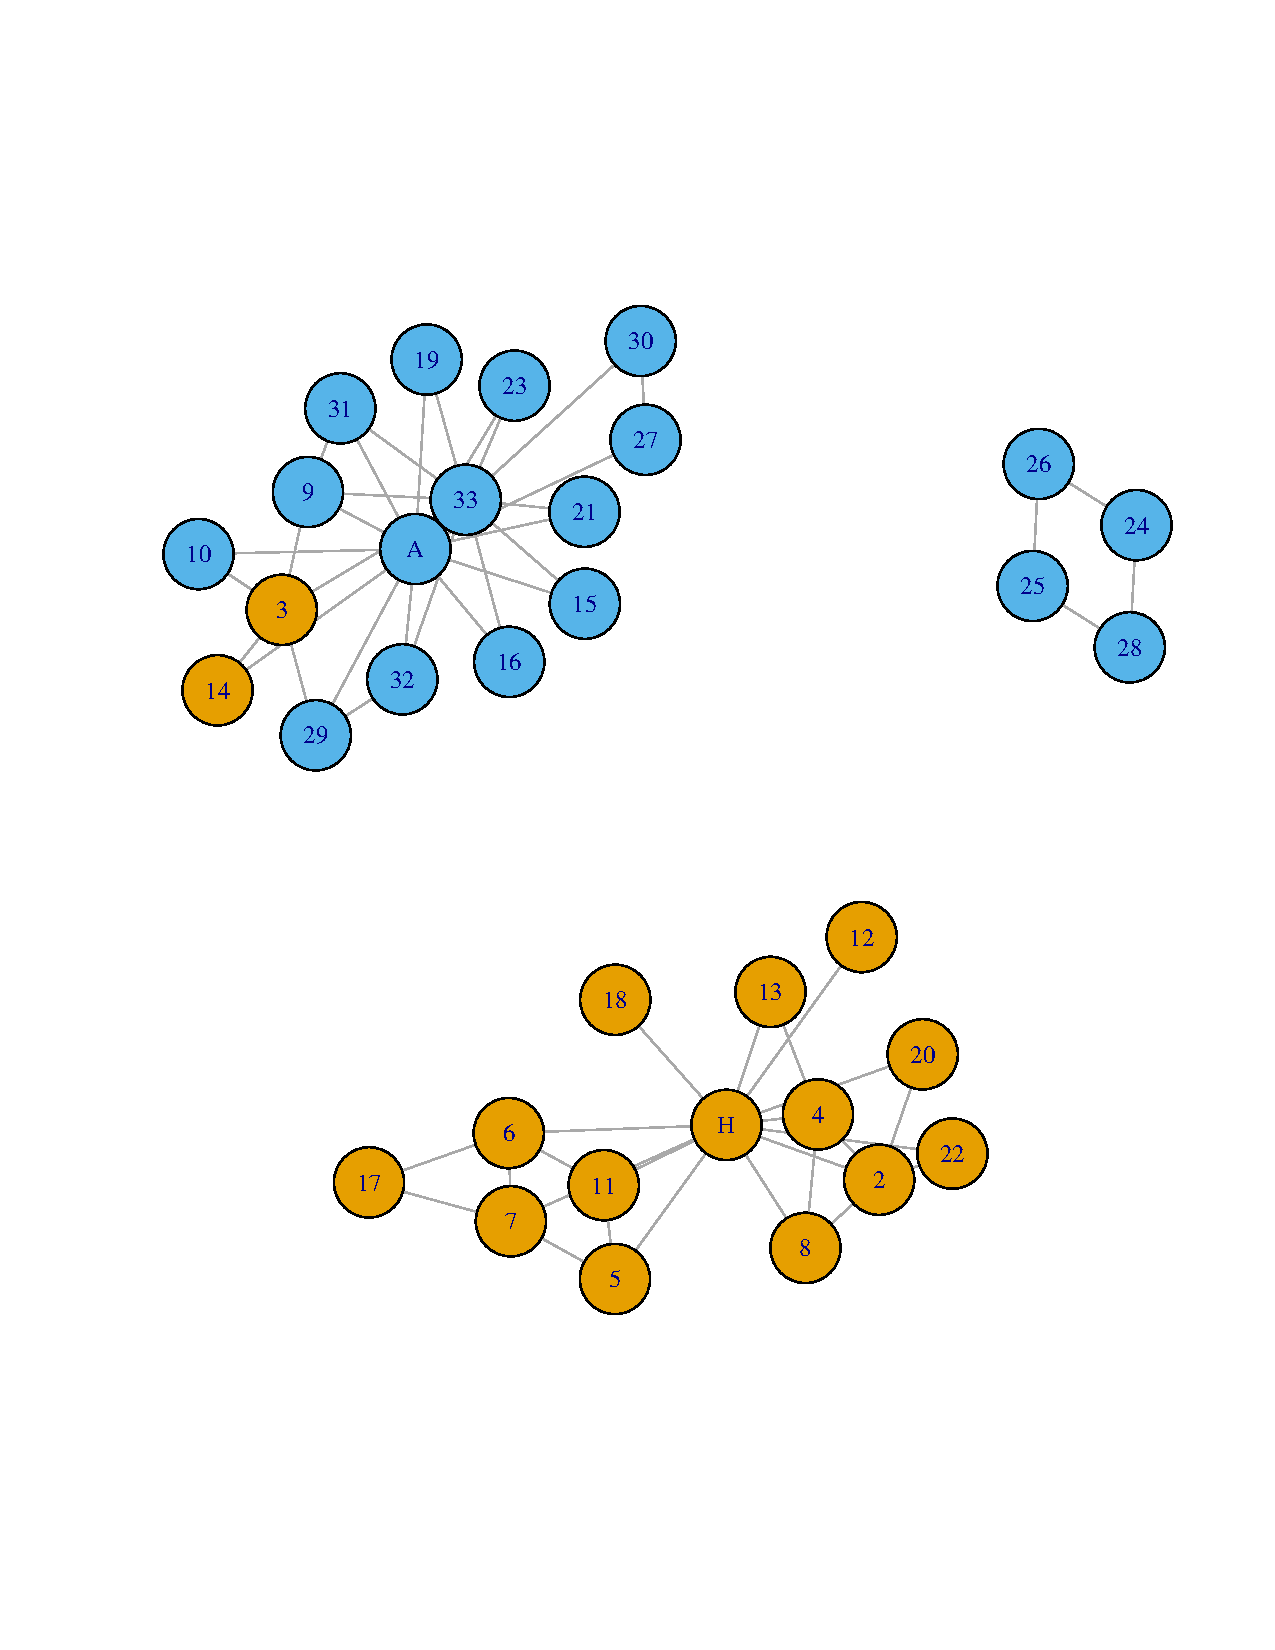
\includegraphics[scale=0.6]{predictedSplit3.pdf}
% \caption{Group split of 3 with Girvan-Newman algorithm from karateClub.R}
% \label{fig:split3}
% \end{figure}

\clearpage

% =================================
% 6th question
% =================================

\section*{6}

\subsection*{Question}

\begin{verbatim}
6.  Re-run questions 1-4, but this time instead of using the 98 
"random" blogs, use 98 blogs that should be "similar" to:

http://f-measure.blogspot.com/
http://ws-dl.blogspot.com/

Choose approximately equal numbers for both blog sets (it doesn't
have to be a perfect 49-49 split, but it should be close).  
Explain in detail your strategy for locating these blogs.  

Compare and contrast the results from the 98 "random" blogs and 
the 98 "targeted" blogs. 
\end{verbatim}

\subsection*{Answer}

\begin{center}
\Huge{NOT ATTEMPTED}
\end{center}


\clearpage


\clearpage


% =================================
% Bibliography
% =================================

\begin{thebibliography}{9}
\bibitem{github}
Atkins, Grant. ``CS532 Assignment 8 Repository'' Github. N.p., 23 March 2017. Web. 23 March 2017.\url{https://github.com/grantat/cs532-s17/tree/master/assignments/A8}.
\bibitem{collectiveIntell}
Segaran, Toby. ``Programming Collective Intelligence''. O' Reilly, 2007. Web. 6 April 2017. \url{http://shop.oreilly.com/product/9780596529321.do}.
\end{thebibliography}

\end{document}